% ----------------------------------------------------------------------
\renewcommand{\CurrentProgressBarIs}{\TwoOfFive}
% ----------------------------------------------------------------------
\begingroup
% \setbeamercolor{normal text}{bg=black}
\setbeamercolor{background canvas}{bg=mLightBrown!10}
\begin{frame}[t,plain]{2. Biomedical text classification (BioTC)}
\end{frame}
\endgroup
% ----------------------------------------------------------------------
\begingroup
\setbeamercolor{background canvas}{bg=mLightBrown!10}
\begin{frame}[t]{2. Biomedical text classification (BioTC)}

\centering
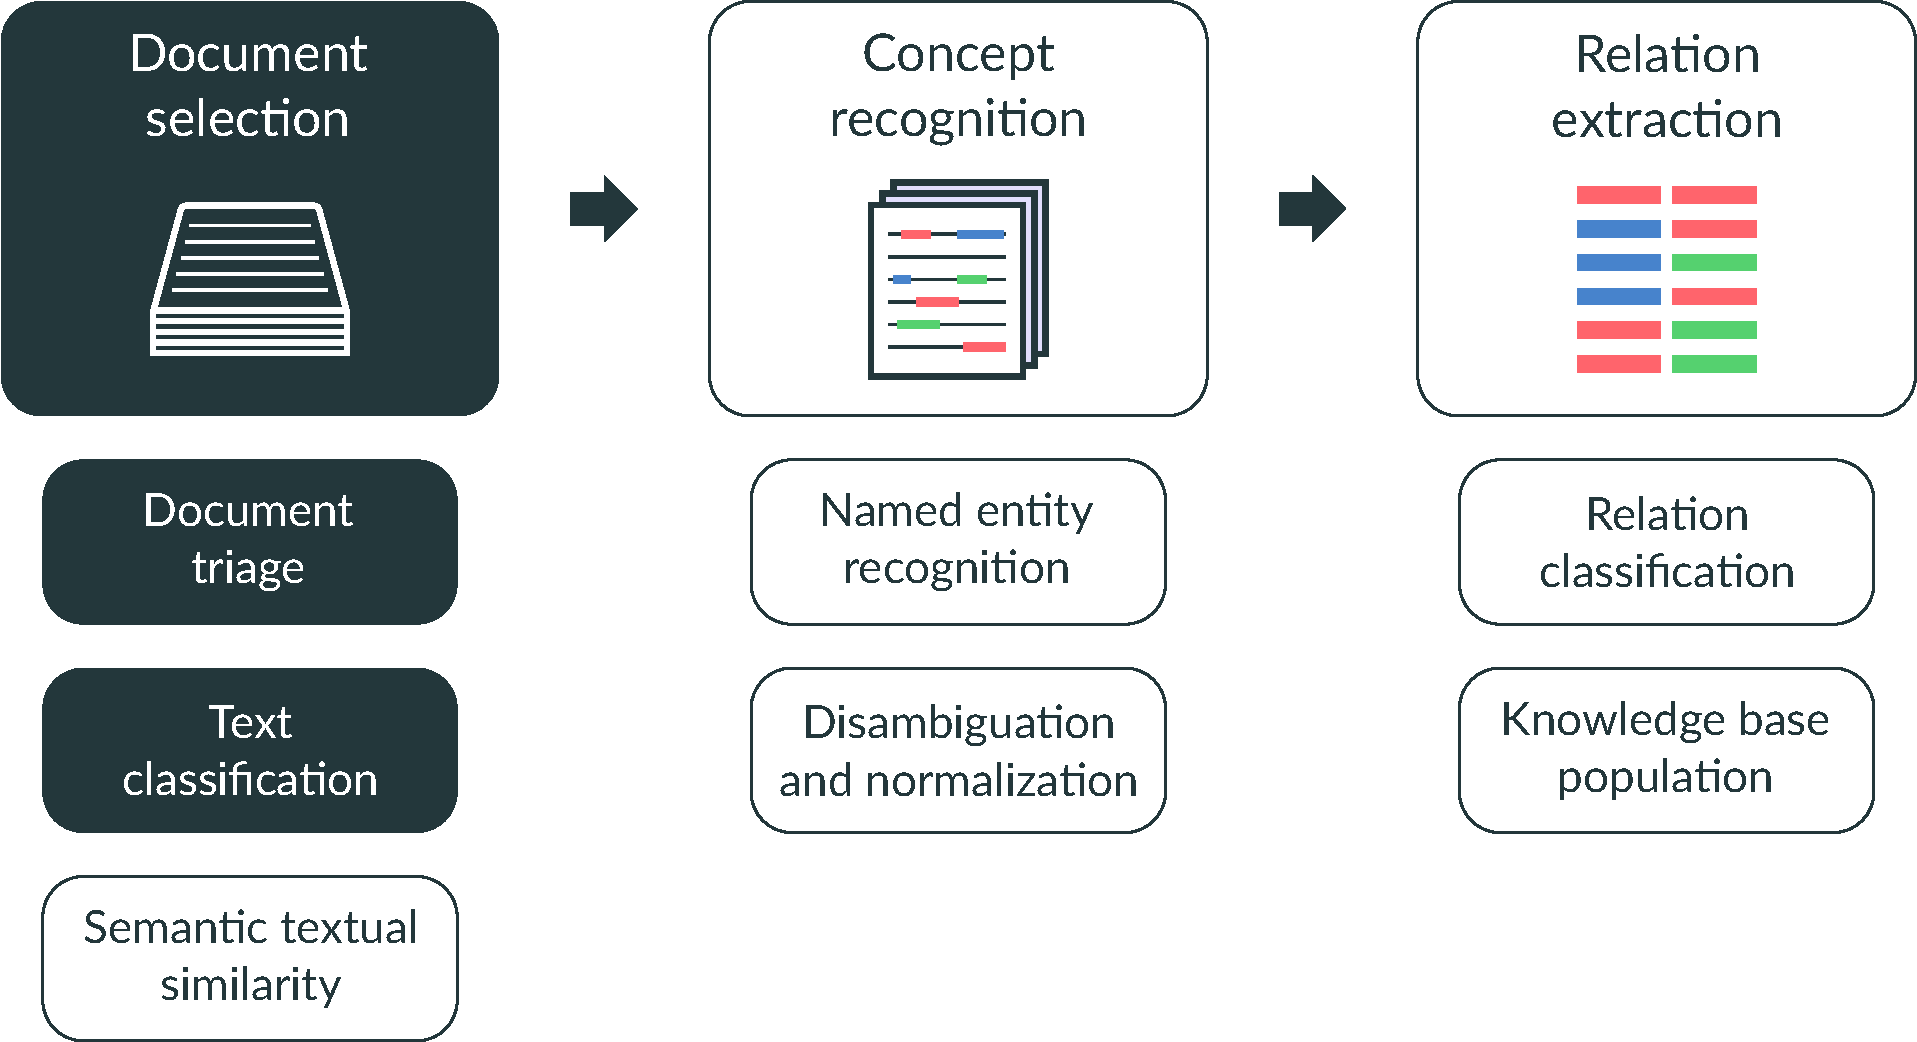
\includegraphics[width=0.80\textwidth]{img/biomedical-information-extraction/v3/011.pdf}%

\end{frame}
\endgroup
% ----------------------------------------------------------------------
\begin{frame}[t]{BioTC: Literature triage for precision medicine}

% \centering
% \vspace*{4mm}

\small

% Remove indentation on itemize.
% https://tex.stackexchange.com/questions/450312/latex-beamer-remove-indent-in-itemize
% \settowidth{\leftmargini}{\usebeamertemplate{itemize item}}
\settowidth{\leftmargini}{7.}
%% \addtolength{\leftmargini}{\labelsep}

\begin{itemize}

\item
BioCreative VI Precision Medicine task dataset

\item
Identify articles describing protein--protein interactions affected by genetic mutations

\end{itemize}

\medskip

\begin{center}
\begin{tabular}{D{16mm}G{20mm}G{20mm}G{20mm}}
Partition & Abstracts & Positive & Negative\\
\midrule
Training  & 4082 & 1729 & 2353\\
Test      & 1427 &  704 &  723\\
\end{tabular}
\end{center}

\vspace*{4mm}

\flushleft
\fontsize{5pt}{6pt}\selectfont
\begin{tabular}{@{}l@{\hskip2pt}l}
Source: & Doğan, Kim, Chatr-Aryamontri, Wei, Comeau, and Lu (October 2017).\\
& \textit{Overview of the BioCreative VI Precision Medicine Track}. BioCreative VI Workshop.\\
& \url{https://biocreative.bioinformatics.udel.edu/tasks/biocreative-vi/track-4/}
\end{tabular}

\end{frame}
% ----------------------------------------------------------------------
\begin{frame}[t]{BioTC: BioCreative VI Precision Medicine task}

\renewcommand*{\arraystretch}{0.5}

% \vspace*{-1mm}

% \footnotesize
\scriptsize

\begingroup
\begin{tabular}{l}
\textbf{Classical machine learning}\\
\midrule
Word embeddings (average) $\cdot$ Traditional classifiers (k-NN, LR, MLP)\\
\end{tabular}
\endgroup

\vspace*{6mm}

\begingroup
\begin{tabular}{l}
\textbf{Deep learning}\\
\midrule
Word embeddings (concatenation) $\cdot$ Convolutional recurrent neural networks\\
\end{tabular}
\endgroup

\vspace*{4mm}

% \footnotesize % 9pt
% \scriptsize % 8pt
% \fontsize{7.5pt}{9.0pt}\selectfont
% \fontsize{7.0pt}{8.4pt}\selectfont
\tiny % 6pt
% \fontsize{5pt}{6pt}\selectfont
% \fontsize{4pt}{4.8pt}\selectfont

\newcommand{\minorscriptsize}{\fontsize{7.0pt}{8.4pt}\selectfont}

\renewcommand*{\arraystretch}{1.0}
\setlength{\tabcolsep}{4pt}%

\begin{columns}[t,totalwidth=\textwidth]

\begin{column}{0.00\textwidth}%
% Nothing, but added just to add left empty space...
\end{column}

\begin{column}{0.20\textwidth}
\begin{tabular}{l@{\hskip0pt}l@{\hskip0pt}l@{\hskip0pt}l}
\multicolumn{4}{l}{\minorscriptsize\textbf{System 1}}\\
\midrule
&                         & \hphantom{0} & Embedding layer\\
&                         &              & Dropout\\
& \multicolumn{1}{l|}{3x} &              & Convolutional layer\\
& \multicolumn{1}{l|}{}   &              & ReLU activation\\
& \multicolumn{1}{l|}{}   &              & Average pooling\\
&                         &              & Bidirectional LSTM\\%*
&                         &              & Dense layer\\
&                         &              & Sigmoid activation\\%[24pt]
\\
\\
% \multicolumn{4}{l}{* Long short-term memory}
\end{tabular}
\end{column}

\newcommand{\mybullet}{\raisebox{0.6pt}{$\bullet$}}
\begin{column}{0.20\textwidth}
\begin{tabular}{l}
{\minorscriptsize\textbf{System 2}}\\
\midrule
\mybullet\ System 1\\
\mybullet\ Self-training approach\\
\hphantom{\mybullet\ }BioCreative III PPI corpus\\
\\
\\
\\
\\
\\
\\
\\
\end{tabular}
\end{column}

\begin{column}{0.30\textwidth}
\begin{tabular}{l@{\hskip0pt}l@{\hskip0pt}l@{\hskip0pt}l}
\multicolumn{4}{l}{\minorscriptsize\textbf{System 3}}\\
\midrule
&                         & \hphantom{0} & Embedding layer\\
&                         &              & Dropout\\
& \multicolumn{1}{l|}{3x} &              & Convolutional layer\\
& \multicolumn{1}{l|}{}   &              & ReLU activation\\
& \multicolumn{1}{l|}{}   &              & Average pooling\\
& \multicolumn{1}{l|}{}   &              & Dropout\\
&                         &              & Bidirectional LSTM\\%*
& \multicolumn{1}{l|}{2x} &              & LSTM\\%*
&                         &              & Dense layer\\
&                         &              & Sigmoid activation\\%[24pt]
% \multicolumn{4}{l}{* Long short-term memory}
\end{tabular}
\end{column}

\end{columns}

\end{frame}
% ----------------------------------------------------------------------
\begin{frame}[t]{BioTC: BioCreative VI Precision Medicine task}

% \centering
\footnotesize
% \scriptsize

% \vspace*{2mm}
% \bigskip
\medskip

% \renewcommand*{\arraystretch}{0.9}

\hspace*{10mm}%
\begin{tabular}{E{40mm}T{19mm}T{19mm}T{19mm}}

& Precision & Recall & F1-score\\

\midrule\addlinespace[6pt]

\multicolumn{4}{l}{\textit{Classical machine learning}}\\

\hspace*{20mm}k-NN (k=99) & 0.618 & 0.553 & 0.582\\
\hspace*{20mm}LR          & 0.674 & 0.546 & 0.603\\
\hspace*{20mm}MLP         & 0.606 & 0.578 & 0.592\\[10pt]

\multicolumn{4}{l}{\textit{Deep learning}}\\

\hspace*{20mm}System 1 & 0.637 & 0.681 & \leavevmode\alert{0.651}\\
\hspace*{20mm}System 2 & 0.640 & 0.692 & \leavevmode\alert{0.664}\\
\hspace*{20mm}System 3 & 0.698 & 0.735 & \leavevmode\alert{\textbf{0.715}}\\

\end{tabular}

\vspace*{8mm}

* 5-fold cross-validation on training set

\end{frame}
% ----------------------------------------------------------------------
\begin{frame}[t]{BioTC: BioCreative VI Precision Medicine task}

% \centering
% \footnotesize % 9pt
% \scriptsize % 8pt
\fontsize{7.5pt}{9.0pt}\selectfont
% \fontsize{7.0pt}{8.4pt}\selectfont
% \tiny % 6pt
% \fontsize{5pt}{6pt}\selectfont
% \fontsize{4pt}{4.8pt}\selectfont

% \vspace*{2mm}
% \bigskip
% \medskip
% \smallskip

\renewcommand*{\arraystretch}{1.05}

\newcommand{\etal}{\textit{et al.}}

% \hspace*{10mm}%
\begin{tabular}{rD{40mm}lrrrr}

Rank & \multicolumn{2}{l}{Work} & \alert{Average precision} & Precision & Recall & \alert{F1-score}\\

\midrule

% 1.  Team 418
% 2.  Team 421
% 3.  Team 374 (ours)
% 4.  Team 419
% 5.  Team 433
% 6.  Team 420
% 7.  Team 375
% 8.  Team 414
% 9.  Team 405
% 10. Team 379

1  & \multicolumn{2}{l}{Fergadis, Baziotis, Pappas \etal}  & 0.7158 & 0.6289 & 0.7656 & 0.6906\\
2  & \multicolumn{2}{l}{Luo, Yang, Lin, and Wang}          & 0.7253 & 0.6073 & 0.7997 & 0.6904\\
\textbf{3} & \textbf{Matos and Antunes} & \alert{\textbf{System 2}} & \alert{\textbf{0.6677}} & \textbf{0.5700} & \textbf{0.8736} & \alert{\textbf{0.6898}}\\
           & \textbf{(ours)}            & \alert{\textbf{System 1}} & \alert{\textbf{0.6616}} & \textbf{0.5864} & \textbf{0.8338} & \alert{\textbf{0.6886}}\\
           &                            & \alert{\textbf{System 3}} & \alert{\textbf{0.6929}} & \textbf{0.6070} & \textbf{0.7898} & \alert{\textbf{0.6864}}\\
4  & \multicolumn{2}{l}{Chen, Singh, Jue, Wang \etal}      & 0.5797 & 0.5713 & 0.8253 & 0.6752\\
5  & \multicolumn{2}{l}{Qu, Steppi, Hao, Wang, Lung \etal} & 0.6632 & 0.5413 & 0.8835 & 0.6713\\
6  & \multicolumn{2}{l}{Tran and Kavuluru}                 & 0.6439 & 0.5438 & 0.8736 & 0.6703\\
7  & \multicolumn{2}{l}{Chen, Panyam, Elangovan \etal}     & 0.6744 & 0.5361 & 0.8849 & 0.6677\\
8  & \multicolumn{2}{l}{Altınel, Hüsünbeyi, and Özgür}     & 0.5077 & 0.5022 & 0.9801 & 0.6641\\
9  & \multicolumn{2}{l}{Team 405}                          & 0.5871 & 0.5484 & 0.5710 & 0.5595\\
10 & \multicolumn{2}{l}{Wang, Shen, Elayavilli, Liu \etal} & 0.4904 & 0.4649 & 0.3480 & 0.3981\\

\end{tabular}

\vspace*{5mm}

* Official test set results

\end{frame}
% ----------------------------------------------------------------------
